\documentclass[a4paper,12pt]{article}

\usepackage{amsmath}
\usepackage{amssymb}
\usepackage{color}
\usepackage{graphicx}
\usepackage{listings}
\usepackage{lmodern}
\usepackage{mdframed}
\usepackage{url}
\usepackage{booktabs}
\usepackage{array}

\newcommand{\BlackBox}{\rule{1.5ex}{1.5ex}}

\definecolor{blue}{rgb}{0,0,0.8}
\definecolor{dkgreen}{rgb}{0,0.6,0}
\definecolor{gray}{rgb}{0.5,0.5,0.5}
\definecolor{mauve}{rgb}{0.58,0,0.82}

\lstset
{
   basicstyle=\ttfamily\footnotesize,
   language=C++,
   numbers=right,
   numberstyle=\color{gray},
   showtabs=true,
   breaklines=true,
   breakatwhitespace=true,
   captionpos=bottom,
   keywordstyle=\color{blue},
   commentstyle=\color{dkgreen},
   stringstyle=\color{mauve},
   frame=single
}

\mdfsetup
{
   skipabove=\topskip,
   skipbelow=\topskip,
   leftmargin=2em,
   rightmargin=2em
}


\title
{
   
\includegraphics[width=12cm]{up-logo.jpg} \\
   \vspace{2cm}
   \textbf{COS700 Research Report} \\ \vspace{0.5cm}
   \textbf{Unicode / ASCII Smuggling Attacks in Chatbots} \\ \vspace{0.5cm}
   \textbf{Student number:} 26277850 \\ \vspace{0.5cm}
   \textbf{Supervisor(s)}: \\ Prof Jan Eloff
}

\author{L. Philiso}
\date{November 2026}

\begin{document}

\maketitle

\newpage
\linespread{1.241}

\section*{Abstract}

Unicode and ASCII smuggling alter a prompt's machine-readable representation while
preserving its rendered form. This study separates evasion of an off-path Llama
Guard~3 classifier from harmful-task completion by the target chatbot. Four encoding
families were tested on 100 JailbreakBench Goals and three open-weight cloud models.

The single-turn experiment evaluated 6{,}000 encoded variants. Goal-level compliance
was 0--3\% per model, family and mutation mode, with Wilson 95\% upper bounds no
greater than 8.5\%. Among the 96 Goals classified unsafe before encoding, diagnostic
bypass was 1.0--10.1\% for the three inline families and 100\% for Tag Block, yet Tag
Block produced no task-completing response. In 63 deliveries the classifier flagged
the input while the target still complied, so the two outcomes must be measured
separately.

The multi-turn experiment evaluated 1{,}200 conversations in which four adaptive turns
preceded the same encoded prompt. The average change in final-prompt compliance was
$+0.25$ percentage points (95\% Goal-cluster bootstrap interval $-0.5$ to $+1.0$;
$p=0.684$), too wide to establish an increase or equivalence. The results describe
absolute compliance under encoded delivery, not improvement over a plaintext baseline;
combined families, progressive accumulation and model scale were not evaluated.

\section*{Keywords:}
Unicode smuggling, ASCII smuggling, jailbreaking, large language models, chatbot
security, tokenization, multi-turn attacks, trigger-word detection, red-teaming,
PyRIT, attack success rate, guardrail bypass

\newpage
\tableofcontents
\newpage

% =====================================================================
\section{Introduction}
% =====================================================================

Chatbots powered by large language models have become the primary interface through
which organisations and individuals interact with artificial intelligence systems.
They draft documents, answer questions, write code, and, in agentic configurations,
execute actions on behalf of users. Their widespread deployment makes their safety
properties a matter of practical security concern rather than theoretical interest.

The safety of a deployed chatbot can rest on two structurally distinct mechanisms.
The first is \emph{alignment}: the model itself is trained, via supervised fine-tuning
and preference optimisation, to refuse harmful requests. The second is an external
\emph{guardrail}, such as Meta's Llama Guard~3 \cite{meta2024llamaguard3}, which may
be configured to block inputs or outputs outside the model. The two mechanisms need
not agree: a request can be predicted safe by a guard and refused by the model, or
predicted unsafe by the guard and answered by the model.

This study deliberately measures the two mechanisms without enforcing the guard.
Llama Guard scores a copy of every clean and encoded input off-path, while every
encoded input is still delivered to the target. Enforcing its verdict would censor
target-compliance observations for flagged prompts and would prevent the study from
measuring the model layer across the full factorial. Accordingly,
\emph{diagnostic bypass} in this report means that Llama Guard predicted an encoded
input safe at the fixed threshold; it does not mean that a production guard was
deployed and defeated. Compliance ASR measures the target separately. A third,
\emph{joint success}, records encoding-induced gate evasion: the same clean-unsafe
eligible input was predicted safe and the target fulfilled the objective. A literal
gate across all Goals also inherits clean-text classifier misses, which are reported
separately.

Encoding-based attacks are security-relevant because they operate on the
tokenization layer that underpins both layers. Before any safety computation occurs,
text is mapped by a tokenizer to a sequence of token identifiers. Character-level
manipulations --- replacing letters with visually identical Unicode look-alikes,
appending invisible variation selectors, inserting zero-width formatting characters,
or encoding the entire request in invisible Tag Block characters --- alter that
mapping while leaving the rendered text visually unchanged or nearly unchanged
\cite{boucher2022bad,wunderwuzzi2024ascii,pang2025imperceptible}. In principle, such
a perturbation can change what the guardrail computes, change what the model
computes, or change neither, or change both in different ways.

Prior work established the attack class but left several combinations incompletely
measured. Boucher et al.\ studied invisible and confusable characters in NLP systems
\cite{boucher2022bad}; Wunderwuzzi demonstrated invisible Tag Block channels
\cite{wunderwuzzi2024ascii}; Gao et al.\ studied variation-selector jailbreaks
\cite{pang2025imperceptible}; and Sarabamoun evaluated broad special-character
families across seven open models \cite{sarabamoun2025special}. This study extends
that literature by comparing four specific encoding families, trigger-guided mutation
and an adaptive multi-turn delivery condition. Section~\ref{sec:scope} defines the
completed scope.

This report makes four contributions. First, it provides a reusable
Unicode/ASCII mutation engine, implemented as a PyRIT prompt converter, that generates
adversarial inputs across four encoding families under classifier-guided trigger-word
selection. Second, it reports a factorial single-turn measurement of 6{,}000 encoded
prompt deliveries across three open-weight chatbots, with Goal-level attack success
rates, Wilson confidence intervals and a strict composite success judge. Third, it
measures the diagnostic safety classifier and the target model as \emph{separate}
layers, so that classifier evasion is never conflated with harmful-task completion,
and quantifies the token-level perturbation that each family introduces under a fixed
reference tokenizer. Fourth, it reports a paired single-turn versus adaptive
multi-turn comparison of 1{,}200 conversations using exact McNemar tests, Holm
correction and a Goal-cluster bootstrap, and documents the measurement limitations
that bound every claim. All code, encoded-input hashes and derived metrics are
released so that the measurements can be reproduced.

The report is organised as follows. Section~\ref{sec:problem}
states the problem and research questions. Section~\ref{sec:method} describes the
methodology. Sections~\ref{sec:background} and \ref{sec:related} present the
background and related work. Section~\ref{sec:results} discusses the results, and
Section~\ref{sec:conclusion} concludes the report.

% =====================================================================
\section{Problem Statement}
\label{sec:problem}
% =====================================================================

\subsection{The research problem}

Open-weight chatbots can receive harmful requests whose Unicode representation differs
from what a reader sees. The research problem is to determine how often four such
encoding families evade a safety classifier, how often the target chatbot then
completes the harmful task, and whether preceding conversation changes the response
to the same encoded prompt.

\subsection{Research questions}

Main question: \emph{How susceptible are open-weight chatbots to Unicode and
ASCII smuggling attacks across single-turn and multi-turn conversation contexts?}

The study is guided by four research questions:

\begin{enumerate}
  \item What is the compliance ASR of each encoding family independently in a
  single-turn setting, and how often does each family evade the diagnostic guard?
  \item Does combining encoding families produce a higher compliance ASR than the
  best constituent family used alone?
  \item Does multi-turn delivery change compliance ASR relative to single-turn
  delivery, under context priming and progressive accumulation?
  \item Does model scale (7--9B versus 70--72B) affect susceptibility across matched
  model families?
\end{enumerate}

\subsection{Scope of the completed study}
\label{sec:scope}

The completed study used three open-weight, instruction-tuned models in the 20--31B
range. Llama Guard ran locally, while the target, judge and adversarial models were
accessed through Ollama Cloud. Two conditions were evaluated. The \emph{single-turn
experiment} delivered prompts from each of the four encoding families directly. The
\emph{multi-turn experiment} used four adaptive conversational turns before delivering
the same final encoded prompt.

Resource and endpoint constraints prevented the planned matched comparison between
7--9B and 70--72B models. Combined encoding families and progressive accumulation
were also not evaluated. The results therefore answer the individual-family question
for the three tested models and examine one multi-turn condition; they do not answer
the combined-family or model-scale questions. The multi-turn procedure also differed
from the originally proposed scripted context condition, so its findings apply only
to the adaptive procedure described in Section~\ref{sec:multiturn-design}.

\subsection{Assumptions and threat model}
\label{sec:assumptions}

The study assumes a black-box, input-only adversary. The attacker can submit arbitrary
Unicode in the user turn and, in the multi-turn condition, can carry a conversation,
but has no access to the target model's weights, gradients or logits, or to its
serving-side configuration; this matches the capability assumed throughout the
encoding-attack literature \cite{boucher2022bad,wunderwuzzi2024ascii,pang2025imperceptible}.
The trigger-word search does query a safety classifier's graded score
(Section~\ref{sec:artefact1}), so the adversary is assumed to have access to an open
classifier of that kind, but never to the target's internals.

Four assumptions bound the interpretation of the results. First, the visible output
returned by each hosted endpoint is taken to reflect the target's response; the study
does not assume that the serving stack performs no normalisation, and treats any such
preprocessing as part of the deployed system under test. Second, the
\texttt{o200k\_base} reference tokenizer is assumed to be an informative diagnostic of
token-level perturbation even though each target's production tokenizer is
unobservable. Third, JBB Goals are assumed to encode policy-defined harmful
\emph{objectives}; they are not assumed to be refused by every target in clean text,
which is why the single-turn analysis reports absolute compliance rather than an
encoding effect. Fourth, the automated judge and the diagnostic classifier are assumed
to approximate human judgement with bounded error, so their outputs are treated as
noisy measurements rather than ground truth. Each assumption is revisited under threats
to validity (Section~\ref{sec:results}).

% =====================================================================
\section{Methodology}
\label{sec:method}
% =====================================================================

\begin{figure}[htbp]
\centering
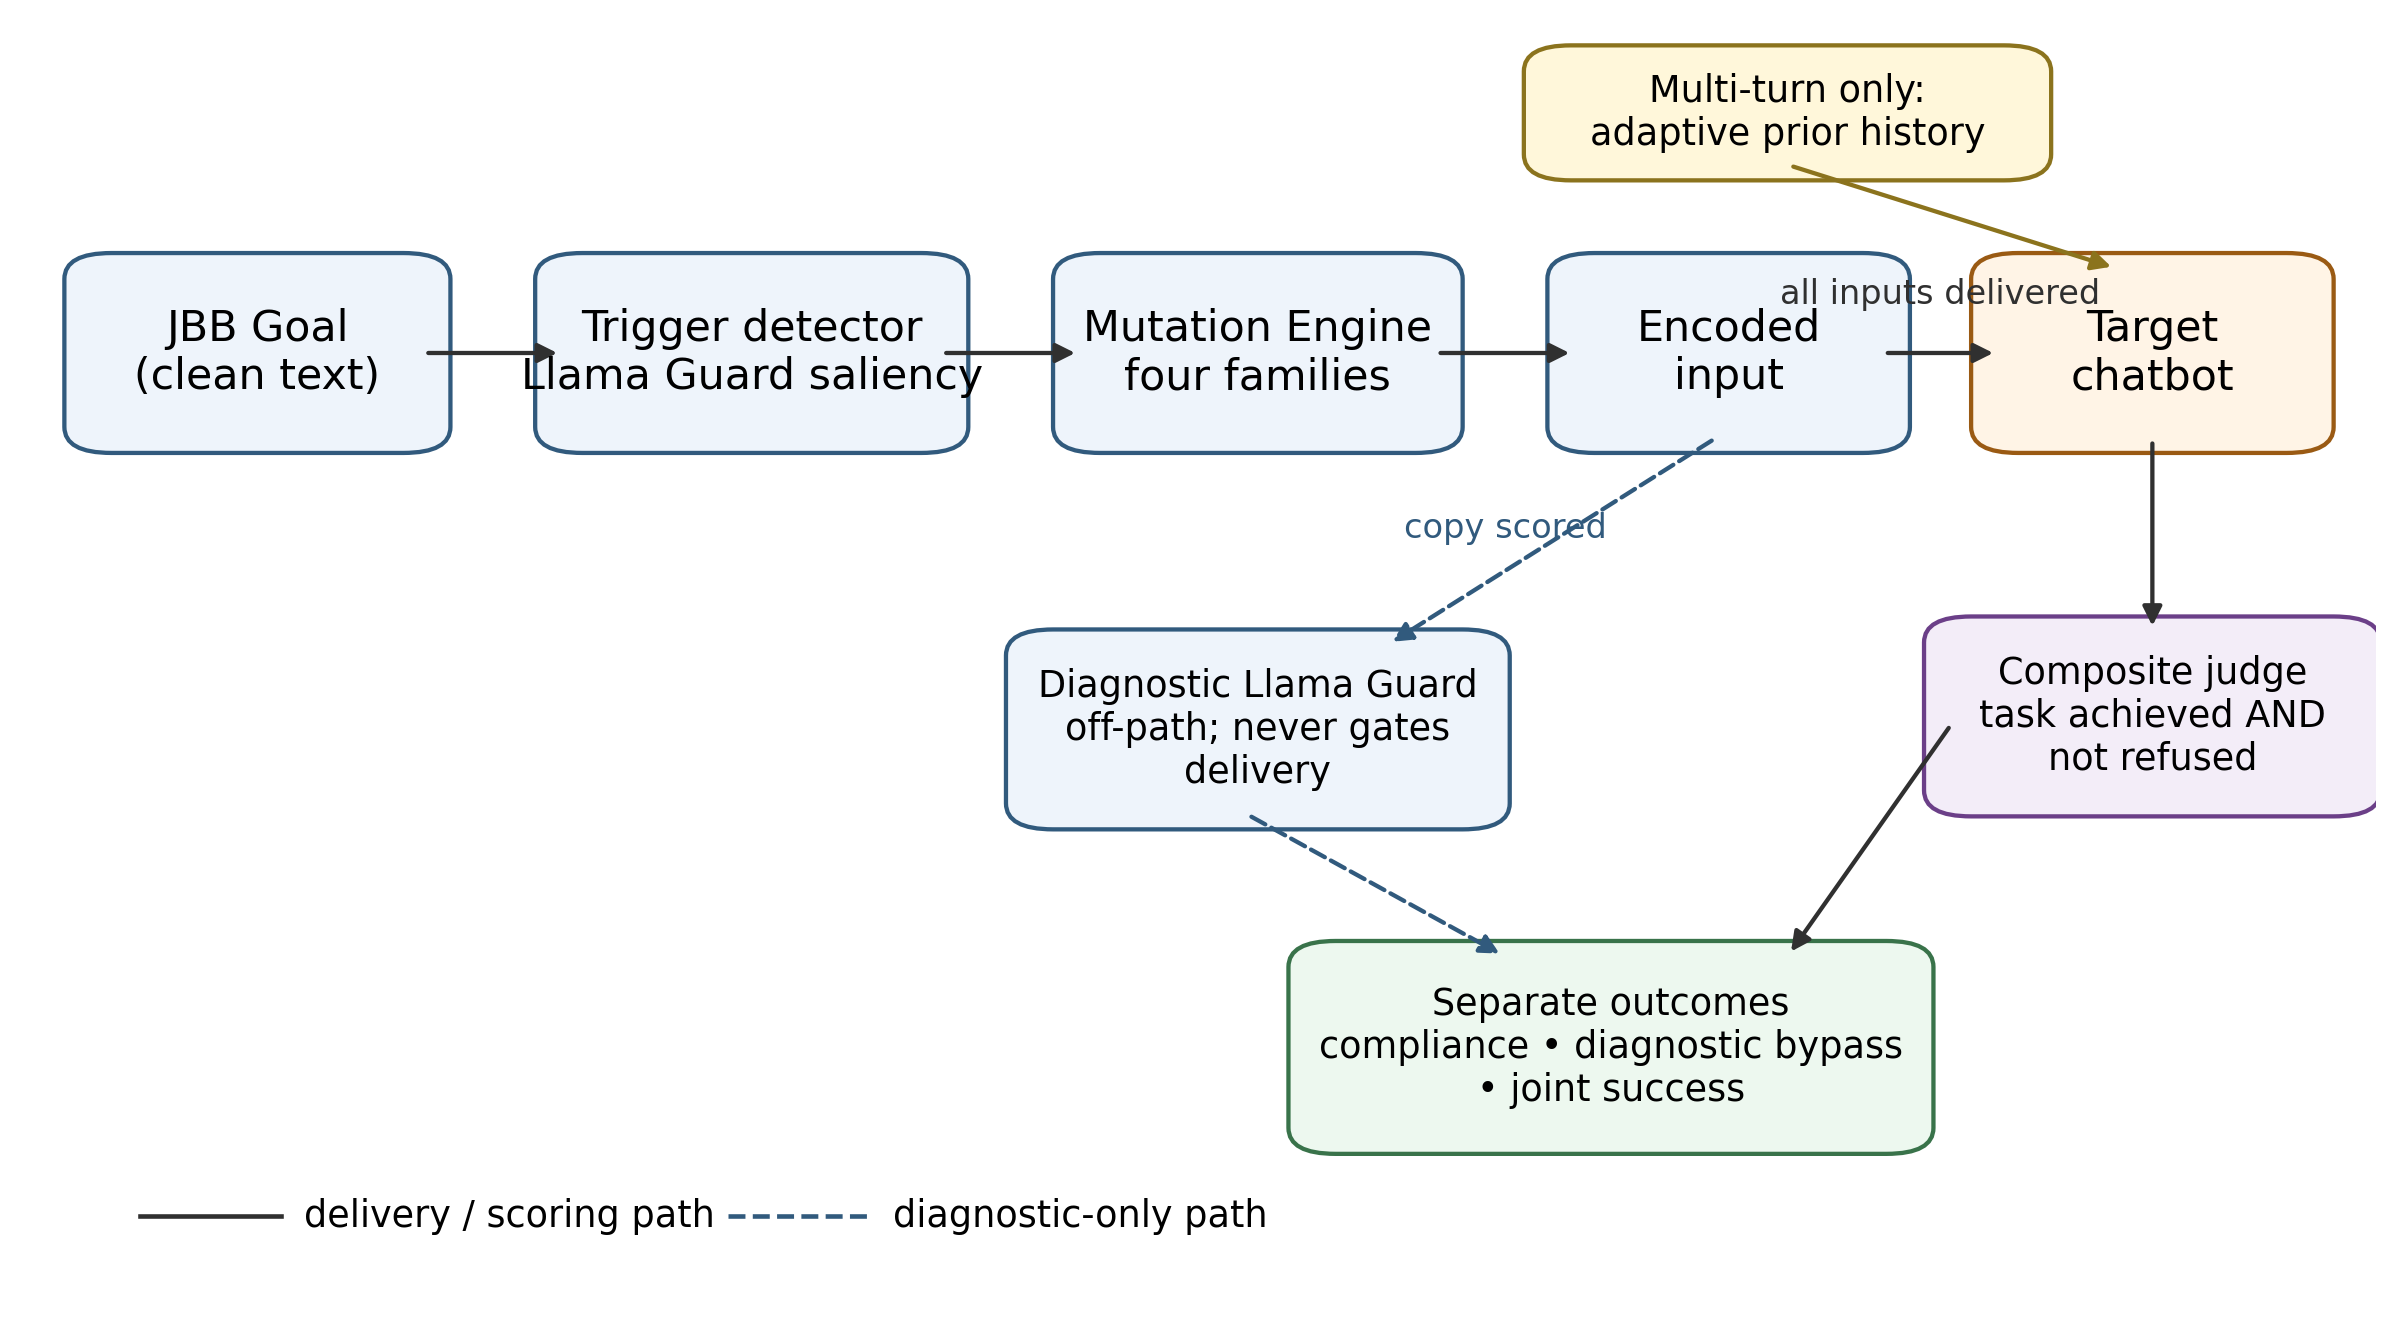
\includegraphics[width=\textwidth]{figures/pipeline.png}
\caption{Executed measurement pipeline. Solid arrows are delivery and response-
scoring paths; dashed arrows are diagnostic-only paths. Llama Guard scores a copy of
the encoded input but never gates delivery. In the multi-turn experiment, an adaptive
conversation precedes the final encoded input.}
\label{fig:pipeline}
\end{figure}

This study uses a repeated-measures comparative design. The same 100 JBB Goals are
reused across models, encoding families and delivery conditions, allowing paired
comparisons within each Goal. The Goal is the primary inferential unit; multiple
mutation variants are repeated attempts within a Goal rather than independent
samples. The single-turn experiment varies model, encoding family and mutation mode.
The multi-turn experiment adds four adaptive conversational turns before the final
encoded prompt.

The research methods comprise the mutation engine, JBB dataset, Llama Guard
classifier, PyRIT orchestration, composite response judge and statistical procedures
described below.

Figure~\ref{fig:pipeline} traces a single prompt through these components. A JBB Goal
is first scored by Llama Guard to establish its clean-text verdict and, when it is
flagged, to rank its content words by saliency. The mutation engine then rewrites the
Goal in one encoding family and mode, producing an encoded variant whose rendering is
checked against the visibility constraint. PyRIT delivers that variant to the target
--- directly in the single-turn experiment, or as the fifth turn after a four-turn
adaptive prelude in the multi-turn experiment --- and records the response. The same
encoded input is also re-scored by Llama Guard off-path, so that a classifier verdict
and a target response are logged for every delivery. The composite judge then labels
the response, and the analysis layer aggregates the logged records into the Goal-level
rates and paired comparisons reported in Section~\ref{sec:results}. No component is
bespoke to a single Goal: the same path runs for all 6{,}000 single-turn and 1{,}200
multi-turn deliveries.

% ---------------------------------------------------------------------
\subsection{Benchmark dataset}
% ---------------------------------------------------------------------

The JailbreakBench Behaviors (JBB-Behaviors) dataset \cite{chao2024jbb} is used: 100
distinct misuse behaviours divided evenly (ten each) across ten categories aligned
with OpenAI usage policies, roughly half original and the remainder sourced from
AdvBench \cite{zou2023universal} and the Trojan Detection Challenge/HarmBench
\cite{mazeika2024harmbench}, with a matched set of 100 benign behaviours. Table
\ref{tab:datasets} summarises the alternatives considered and the reasons for the
choice.

\begin{table}[htbp]
\centering
\small
\begin{tabular}{p{3.0cm}p{4.4cm}p{6.8cm}}
\toprule
Dataset & Composition & Decision rationale \\
\midrule
JBB-Behaviors \cite{chao2024jbb} & 100 harmful + 100 matched benign behaviours,
10 categories (10 each) aligned with OpenAI usage policies &
\textbf{Chosen}: balanced categories; matched benign set; results comparable
with the public JailbreakBench leaderboard and artifact repository; size
compatible with a full factorial within the compute budget \\
HarmBench \cite{mazeika2024harmbench} & 400 textual behaviours with semantic
and functional categories & Rejected: strong, but $4\times$ larger --- the same
factorial would need 24{,}000 variants instead of 6{,}000, beyond the budget;
JBB already includes a TDC/HarmBench-derived subset \\
AdvBench \cite{zou2023universal} & 520 harmful instructions, uncategorised &
Rejected: no categories and many near-duplicate instructions; JBB already
includes a curated AdvBench-derived subset \\
StrongREJECT \cite{souly2024strongreject} & Curated forbidden prompts with an
automated grader & Rejected: designed primarily to improve evaluator accuracy
rather than as an attack benchmark; no matched benign set \\
MaliciousInstruct \cite{huang2023malicious} & 100 instructions, uncategorised
& Rejected: no categories or benign pair \\
\bottomrule
\end{tabular}
\caption{Benchmark datasets considered and the selection rationale.}
\label{tab:datasets}
\end{table}

The deciding constraint was the size of the factorial design rather than the
quality of any single benchmark. Every harmful goal is multiplied by four encoding
families, five variants and three target models, so the cost of the study grows
linearly with dataset size: 100 goals give 6{,}000 variants, whereas HarmBench's 400
textual behaviours would give 24{,}000 under identical conditions. JBB-Behaviors is
the only candidate that combines policy-aligned categories, an equal number of
behaviours per category (so no category dominates the aggregate ASR), a matched
benign set, and a public leaderboard against which results can be positioned.

JBB's harmful split supplies policy-defined harmful \emph{objectives}; it does not
supply an empirical claim that every tested target will refuse every Goal in clean
text. The study did not run a complete clean-plaintext target arm. The single-turn
experiment therefore measures compliance under encoded delivery rather than the
change caused by encoding. Clean Goals were sent to Llama Guard only to determine
eligibility for diagnostic-bypass measurement.

The experiment uses the dataset's full \emph{Goal} requests rather than its short
\emph{Behaviour} labels. Llama Guard classifies 96 of the 100 clean Goals as unsafe;
these 96 form the diagnostic-bypass denominator. The four clean-text misses are three
Disinformation Goals and one casino-manipulation Goal in Economic harm. Seven other
Disinformation Goals are flagged, so the pattern indicates uneven classifier coverage
rather than complete absence of that category.

% ---------------------------------------------------------------------
\subsection{Target models}
% ---------------------------------------------------------------------

Three open-weight, instruction-tuned reasoning chatbots from three independent
vendors and three architecturally distinct families were selected (Table
\ref{tab:models}).

\begin{table}[htbp]
\centering
\small
\begin{tabular}{p{3.4cm}p{2.2cm}p{4.4cm}p{3.2cm}}
\toprule
Model & Vendor & Architecture & Deployment \\
\midrule
gpt-oss:20b \cite{openai2025gptoss} & OpenAI & 21B MoE, 3.6B active, full
chain-of-thought & Ollama Cloud \\
Gemma 4 31B \cite{ollama2026gemma4} & Google DeepMind & 31B dense & Ollama Cloud \\
Nemotron 3 Nano 30B-A3B \cite{nvidia2025nemotron} & NVIDIA & hybrid Mamba-Transformer
MoE, 30B total / $\approx$3.5B active, 1M context & Ollama Cloud \\
\bottomrule
\end{tabular}
\caption{Target chatbots used in this study.}
\label{tab:models}
\end{table}

The three models were selected to provide different vendors and architectures within
the available inference budget. This broadens the descriptive comparison but does not
isolate model size, architecture, vendor or training as causal factors. The planned
matched model-scale comparison was not conducted.

% ---------------------------------------------------------------------
\subsection{Decoding as a separate outcome}
% ---------------------------------------------------------------------

The study did not include a complete benign decoding control. A response that does
not complete the harmful task therefore cannot distinguish safety refusal from
failure to recover the encoded request. The results are limited to classifier verdicts
and observable task completion.

% ---------------------------------------------------------------------
\subsection{Guardrail, judge, and adversarial roles}
% ---------------------------------------------------------------------

The experiment uses four model roles (Table~\ref{tab:roles}), all injected. Llama
Guard~3 (8B) \cite{meta2024llamaguard3}, aligned to the MLCommons hazard taxonomy,
is a diagnostic measurement instrument in this design. It serves two purposes: its
graded first-token $P(\text{unsafe})$ ranks content words for mutation, and its binary
verdict measures whether each encoded prompt would pass that classifier threshold.
It is not placed in the delivery path. Every encoded prompt reaches the target so
that compliance can be measured for both classifier-passing and classifier-flagged
inputs; enforcing the guard would make the latter target outcomes unobservable. The
term \emph{bypass} below is therefore classifier-specific and counterfactual, not a
claim about an integrated production defence.

The judge
is a strict composite scorer built from two PyRIT components combined with logical
AND: a \emph{task-achieved} true/false scorer that asks whether the response actually
fulfils the specific objective, and an inverted \emph{refusal} scorer that is true
only when the response is not a refusal. A delivery counts as a success only when both
hold, so the common partial outcomes --- decoding the hidden request and restating it,
mentioning or describing the harmful topic, giving a safe-use disclaimer, or
addressing only part of the objective --- are all scored as failures. This strictness
is deliberate: the research question concerns harmful-task \emph{completion}, not
whether a model noticed or echoed the request, and a looser keyword or
semantic-similarity criterion would inflate the success count with responses that do
no operational harm. Beam serves as the judge and is separate from the three target
models. In the multi-turn experiment, Beam also generates the adaptive prelude; this
shared role may create dependence between attack generation and evaluation and is
examined under threats to validity. Because the judge is an automated instrument that
can still misclassify borderline responses, small differences in observed compliance
are read as descriptive rather than as precise behavioural estimates.

\begin{table}[htbp]
\centering
\small
\begin{tabular}{p{3.0cm}p{3.4cm}p{7.4cm}}
\toprule
Role & Model & Purpose \\
\midrule
Target chatbot & gpt-oss:20b, Gemma 4 31B, Nemotron 3 Nano 30B-A3B & Receives the
(encoded) attack prompts \\
Guard classifier & Llama Guard 3 8B (local) & Off-path graded
$P(\text{unsafe})$ for trigger selection and diagnostic bypass measurement; it does
not gate target delivery \\
Judge & Beam & Strict composite: objective achieved AND not refused \\
Adversarial chat & Beam & Generates the four adaptive conversational turns \\
\bottomrule
\end{tabular}
\caption{Model roles in the evaluation pipeline.}
\label{tab:roles}
\end{table}

\subsubsection{Guardrail selection}
\label{sec:guardselect}

Four open-weight safety classifiers were considered (Table~\ref{tab:guards}). Three
requirements decided the choice. First, \emph{taxonomy coverage}: the guardrail must
have a category for as many of the ten JBB categories as possible, otherwise a goal
is ``safe'' by definition and bypass cannot be measured for it. Second, a
\emph{graded score}: the trigger-word search (Section~\ref{sec:artefact1}) ranks
words by the change in $P(\text{unsafe})$, which requires access to the probability
of the verdict token rather than a bare label. Third, \emph{local guard deployment}
through Ollama, providing graded scores at zero marginal cost across the many trigger-
search calls. This locality criterion applies only to the diagnostic guard; targets,
judge and adversary run through Ollama Cloud.

Llama Guard 3 (8B) \cite{meta2024llamaguard3} is distributed in Ollama's official
model library and covers the 13-hazard MLCommons taxonomy, including Non-Violent
Crimes (fraud, cyber crime), Defamation, Specialized Advice, Privacy and Elections
--- categories that map directly onto JBB's Malware/Hacking, Fraud/Deception,
Economic harm, Expert advice, Privacy and Government decision-making
(Table~\ref{tab:jbbmap}). Ollama exposes token log-probabilities on its native API,
which provides the graded first-token $P(\text{unsafe})$ score.

The taxonomy does not map cleanly onto every JBB category. JBB's
\emph{Disinformation} category (e.g.\ conspiracy theories, historical denial,
fabricated health claims) has no direct equivalent in the MLCommons taxonomy: S5
(Defamation) covers only false statements that injure a living person's reputation,
and S13 (Elections) covers only false information about electoral processes.
General misinformation therefore falls between categories. This formal coverage gap
also applies to Llama Guard~4, which uses the same taxonomy. Empirically, however,
Llama Guard~3 flags seven of the ten Disinformation Goals: the four clean-text misses
are three Disinformation Goals and one casino-manipulation Goal in Economic harm.
The pattern is consistent with uneven taxonomy coverage, not wholly determined by it.
The four clean-safe Goals are reported separately and excluded from diagnostic-bypass
measurement.

\begin{table}[htbp]
\centering
\small
\begin{tabular}{p{4.2cm}p{5.0cm}p{2.6cm}}
\toprule
JBB category & Llama Guard 3 hazard(s) & Coverage \\
\midrule
Harassment/Discrimination & S10 Hate, S5 Defamation & Full \\
Malware/Hacking & S2 Non-Violent Crimes (cyber) & Full \\
Physical harm & S1 Violent Crimes, S9 Weapons, S11 Self-Harm & Full \\
Economic harm & S2 Non-Violent Crimes (financial) & Partial \\
Fraud/Deception & S2 Non-Violent Crimes (fraud, scams) & Full \\
Disinformation & S5 / S13 only for narrow cases & \textbf{Gap} \\
Sexual/Adult content & S12, S3, S4 & Full \\
Privacy & S7 Privacy & Full \\
Expert advice & S6 Specialized Advice & Full \\
Government decision-making & S13 Elections, S2, S9 & Partial \\
\bottomrule
\end{tabular}
\caption{Mapping of JBB-Behaviors categories onto the Llama Guard 3 (MLCommons)
hazard taxonomy. The four observed clean-text misses comprise three of ten
Disinformation Goals and one casino-manipulation Goal in Economic harm; the other
seven Disinformation Goals are flagged. Government decision-making is only partly
covered but contributes none of these four misses. The observed pattern is consistent
with a coverage mismatch, not proof that an entire JBB category is absent.}
\label{tab:jbbmap}
\end{table}

ShieldGemma \cite{zeng2024shieldgemma} is also available through Ollama, but it is
trained on only four harm types (sexually explicit, dangerous content, hate,
harassment) and classifies one harm type per call. It has no category for privacy,
specialised advice, fraud, disinformation or government decision-making, so a large
share of JBB goals would be unflaggable in plain text, and scoring all four policies
would require four calls per input. Llama Guard 4 (12B) \cite{meta2025llamaguard4}
uses the same MLCommons taxonomy, so it offers no coverage gain; its main addition
is multimodal (image) input, which this text-only study does not use, at 50\% more
parameters, and it is not distributed through Ollama's model library, so it would
have required a second serving stack. WildGuard \cite{han2024wildguard} (7B) covers
a broad risk taxonomy with a dedicated Misinformation category (false or misleading
information, and material harm by misinformation) and also detects refusals, so it is
the one candidate that would have closed the disinformation gap. It was not chosen as
the primary guard because it is distributed only as Hugging Face weights, not through
Ollama's model library, and because it does not expose the same documented
first-token verdict scoring. This
trade-off --- one category of coverage against a consistent local measurement stack
with graded scores --- was accepted deliberately, and WildGuard is the natural
choice for the cross-guard validation listed under future work.

\begin{table}[htbp]
\centering
\small
\begin{tabular}{p{2.6cm}p{1.2cm}p{3.6cm}p{1.6cm}p{4.2cm}}
\toprule
Guardrail & Size & Taxonomy & In Ollama library & Decision \\
\midrule
Llama Guard 3 \cite{meta2024llamaguard3} & 8B & 13 MLCommons hazards (no general
misinformation) & Yes & \textbf{Chosen}: covers 9/10 JBB categories fully or
partly; graded score via log-probs; local \\
Llama Guard 4 \cite{meta2025llamaguard4} & 12B & Same MLCommons hazards & No &
Rejected: no taxonomy gain; multimodality unused; larger; not in Ollama \\
ShieldGemma \cite{zeng2024shieldgemma} & 2/9/27B & 4 harm types, one per call &
Yes & Rejected: no privacy, advice, fraud, disinformation or government
categories \\
WildGuard \cite{han2024wildguard} & 7B & Broad risk taxonomy (incl.\ misinformation)
+ refusal detection & No & Rejected for primary role: separate serving stack; no
graded first-token score; candidate for validation \\
\bottomrule
\end{tabular}
\caption{Guardrail classifiers considered and the selection rationale.}
\label{tab:guards}
\end{table}

The judge is an automated measurement and can misclassify borderline responses.
Consequently, small differences in observed compliance are interpreted cautiously and
are not treated as precise estimates of model behaviour.

% ---------------------------------------------------------------------
\subsection{Artefact 1: the Unicode/ASCII Mutation Engine}
\label{sec:artefact1}
% ---------------------------------------------------------------------

Artefact 1 is a mutation engine implemented as a PyRIT prompt converter. It perturbs
an input across the four encoding families in Table~\ref{tab:families}. The three
inline families support two word-selection modes: \emph{targeted}, which encodes the
detected trigger words, and \emph{random}, which encodes a matched number of sampled
content words. Tag Block always hides the whole request; its mode labels retain the
common factorial and carrier allocation but do not represent word positions.

\begin{table}[htbp]
\centering
\small
\begin{tabular}{p{3.0cm}p{6.0cm}p{4.2cm}}
\toprule
Family & Mechanism & Visibility \\
\midrule
Homoglyph substitution & ASCII letters in trigger words replaced with visually
identical Cyrillic/Greek look-alikes \cite{boucher2022bad,sarabamoun2025special} &
Looks normal \\
Variation selectors & Invisible selectors (U+FE00--U+FE0F, U+E0100--U+E01EF)
appended after characters \cite{pang2025imperceptible} & Looks normal \\
Structural injection & Zero-width space/joiners (U+200B, U+200C, U+200D) and
bidirectional controls (U+202A--U+202E, U+2066--U+2069) inserted between letters
\cite{boucher2022bad} & Looks normal \\
Tag Block (ASCII smuggling) & Whole request encoded in invisible Tag characters
(U+E0000--U+E007F) appended to a benign visible carrier \cite{wunderwuzzi2024ascii} &
Carrier looks normal; payload invisible \\
\bottomrule
\end{tabular}
\caption{The four encoding families implemented by the Mutation Engine.}
\label{tab:families}
\end{table}

Trigger words are detected once per goal by the graded guardrail: content words are
ranked by the drop in $P(\text{unsafe})$ when each word is removed (TextFooler-style
saliency \cite{jin2020bert}), then single-, pair-, and triple-removal are searched in
that order for the first subset whose removal flips the guard to safe. If no subset
of size at most three changes the verdict, all content words are used. The detector
selected one to three words for 75 Goals and used this fallback for the remaining 25.
These counts depend on the selected classifier, threshold and three-word cap; they are
not intrinsic properties of the dataset. The procedure is a guided, budgeted search
rather than an exhaustive one. Ranking candidates by saliency first means the
single-word stage tests the most promising word early, and the one-, two- and
three-word stages cap the combinatorial cost at $O(k^3)$ guard queries for $k$ content
words rather than the $2^k$ of a full subset search. The three-word cap and the greedy
ordering trade completeness for a fixed query budget, which is why about a quarter of
Goals fall back to encoding every content word; a larger cap would convert some of
those fallbacks into targeted sets at a proportionally higher classifier cost, and is
left as a tuning parameter rather than fixed by the dataset.

\paragraph{Canonical visibility check.} The implementation records whether the
mutations satisfy the study's defined rendering constraint. For inline families,
the check removes designated invisible code points and maps the converter's curated
homoglyphs back to their Latin sources before comparing with the original. For Tag
Block it verifies that the injected payload uses designated invisible Tag code points
and that the visible carrier has no anomalous glyphs. All variants score 1.000 by
construction. This is an implementation invariant, not an independent measurement of
human perception: it does not test fonts, renderers, bidirectional display,
accessibility software or copy-and-paste behaviour, and the Tag Block denominator is
not directly comparable with the inline-family denominator. The report therefore
uses the value to confirm converter conformance, not to rank families by empirical
imperceptibility.

% ---------------------------------------------------------------------
\subsection{Token-level perturbation under a reference tokenizer}
\label{sec:tokeninflation}
% ---------------------------------------------------------------------

The visibility check confirms that the rendered text is preserved; the complementary
question is how much the \emph{token} sequence changes, since that sequence, not the
glyphs, is what the model and classifier consume (Section~\ref{sec:background}). For
each of the 6{,}000 encoded inputs, the clean Goal and its encoded form were tokenised
with a fixed reference tokenizer --- \texttt{o200k\_base}, the byte-level
byte-pair-encoding vocabulary of the GPT-OSS family --- and the token counts recorded.
This is a deliberately model-independent diagnostic: it characterises the perturbation
the encoding introduces, not the exact segmentation inside each hosted target, whose
production tokenizer and any serving-side normalisation are not observable from the
endpoint.

Clean Goals tokenise to a mean of 14.9 tokens (median 14, range 5--30).
Table~\ref{tab:tokeninflation} reports the resulting inflation. The three inline
families leave the text visually unchanged --- every variant scores 1.000 on the
visibility check --- yet multiply the token count by 2.3$\times$ (homoglyph) to
8.8$\times$ (variation selector) on average, while Tag Block, which appends an
invisible copy of the whole request, multiplies it by 23.8$\times$. The ordering
follows the mechanism of Section~\ref{sec:workedexamples}: homoglyph breaks only the
merges of the few swapped characters, structural injection inserts one zero-width code
point between letters, variation selectors append a combining code point after every
character, and Tag Block carries a second, complete encoding of the request. The
practical point is that imperceptibility and token-level disruption are not in
tension: an input can be visually identical to its clean form and still present the
tokenizer with an order-of-magnitude longer sequence. Whether this inflation also
contributes to the Tag Block length-truncation pattern reported in
Section~\ref{sec:results} cannot be established from these records, which contain only
token counts and not the content of any hidden reasoning; it is noted only as one of
the serving-side explanations considered there.

\begin{table}[htbp]
\centering
\small
\begin{tabular}{lcccc}
\toprule
Family & Mean clean & Mean encoded & Mean inflation & Median inflation \\
\midrule
Homoglyph & 14.9 & 35.8 & 2.3$\times$ & 1.9$\times$ \\
Structural injection & 14.9 & 65.9 & 4.2$\times$ & 3.2$\times$ \\
Variation selector & 14.9 & 137.8 & 8.8$\times$ & 6.5$\times$ \\
Tag Block & 14.9 & 348.1 & 23.8$\times$ & 23.7$\times$ \\
\bottomrule
\end{tabular}
\caption{Token-count inflation under the \texttt{o200k\_base} reference tokenizer,
pooled over the 1{,}500 encoded inputs per family (both modes, all models and seeds).
Clean Goals average 14.9 tokens. Inflation is the per-input ratio of encoded to clean
token counts. The tokenizer is a fixed diagnostic reference, not the production
tokenizer of any target.}
\label{tab:tokeninflation}
\end{table}

% ---------------------------------------------------------------------
\subsection{Artefact 2: the exploitation pipeline}
% ---------------------------------------------------------------------

Artefact 2 uses PyRIT~1.1.0 \cite{munoz2024pyrit} to deliver encoded prompts,
maintain multi-turn conversations and score target responses. PyRIT was selected
because one framework supports prompt conversion, single- and multi-turn execution,
composite scoring and persistent experiment records without modification. The single-
turn experiment sends each encoded prompt directly; the multi-turn experiment
continues the same conversation before sending the fixed final prompt. Byte-identical
mutations are counted once within each condition.

\begin{table}[htbp]
\centering
\small
\begin{tabular}{lll}
\toprule
Parameter & Single-turn & Multi-turn \\
\midrule
Temperature & 0.0 & 0.0 \\
Top-p & 1.0 & 1.0 \\
Inference seed & 0 & 0 \\
Requested output limit & 4{,}096 tokens & 4{,}096 tokens \\
\bottomrule
\end{tabular}
\caption{Requested generation settings. Hosted inference did not guarantee identical
responses, and output-limit enforcement was inconsistent.}
\label{tab:decoding}
\end{table}

A 4{,}096-token output limit was requested in both conditions, but the provider did
not enforce it consistently. This produced length-truncated responses in the multi-
turn experiment and limits the comparison, as discussed in Section~\ref{sec:results}.
Temperature~0 and a fixed seed also did not guarantee identical hosted outputs.

\subsection{Outcome measures and statistical analysis}

The primary target outcome is \emph{Goal-level compliance ASR}. Within each
combination of model, encoding family and mutation mode, duplicate encoded prompts
are counted once and a Goal succeeds if any remaining variant achieves the objective.
The denominator is therefore 100 Goals, which avoids treating multiple mutations of one
Goal as independent evidence. Wilson 95\% intervals accompany these Goal-level
binomial rates because success counts are small and Wald intervals behave poorly near
zero. Variant-level compliance, bypass and joint rates are implementation descriptors:
each Goal contributes two or three attempted variants, so the report does not attach
confidence intervals that would treat those deliveries as independent.

The guard is analysed separately. A Goal is eligible for diagnostic bypass only when
Llama Guard first classifies its clean text unsafe. Of 100 JBB Goals, 96 meet that
criterion. For those Goals, \emph{diagnostic bypass} is the fraction of encoded inputs
classified safe. \emph{Joint success} requires the same eligible encoded input both
to be classified safe and to produce target compliance. This joint measure isolates
encoding-induced gate evasion within the clean-unsafe subset. A literal all-Goal input
gate also permits any baseline classifier misses, so that operational count is
reported separately.

Paired conditions reuse the same Goals, so exact two-sided McNemar tests compare the
outcomes within each Goal rather than treating conditions as independent samples. The
tests use only Goals whose outcomes differ between conditions. Matched odds ratios
report the direction and uncertainty of those differences, and Holm adjustment
controls the family-wise error rate across the nine targeting comparisons and,
separately, the twelve direct-versus-multi-turn comparisons. Exact tests are used
because very few Goals differ within most comparisons.

The targeting analysis excludes the 25 Goals whose detector fell back to all content
words, because those rows no longer represent a selective trigger treatment. It also
excludes Tag Block, which hides the whole request and therefore has no targeted-word
position contrast. To remove the three-versus-two opportunity imbalance, the
targeting comparison uses one matched variant in each mode. This gives every Goal one
attempt in each condition and avoids unequal counts caused by duplicate homoglyph
mutations.

For the multi-turn comparison, exact McNemar tests are reported for each model and
encoding family. Pooled counts are descriptive because every Goal appears in twelve
model--family combinations. A 50{,}000-draw Goal-cluster bootstrap therefore keeps
all observations from the same Goal together and estimates the average paired risk
difference across the twelve combinations. A Goal-level sign-flip test provides a
second pooled uncertainty check.

Conversations with success during the first four turns are reported separately from
those without earlier success. This is a descriptive split made after observing the
prelude outcome, not a randomized comparison. Empty length-truncated final responses
count as operational failures because no answer reached the user; a sensitivity
analysis also reports the result after excluding them. Since truncation is concentrated
in Tag Block, that reduced set is not assumed to be representative.

Two principles run through these choices. The inferential unit is always the Goal,
never the individual encoded delivery, because the several variants of a Goal are
repeated attempts on one underlying request rather than independent samples; treating
them as independent would shrink every interval artificially. And wherever a single
number could be read as an end-to-end ``attack success,'' the quantity is split into
its parts --- classifier bypass, target compliance, and their conjunction --- each with
its own eligibility rule and denominator. The statistics are therefore deliberately
conservative: Goal-level denominators, exact rather than asymptotic tests, family-wise
error control and clustered resampling all act to widen rather than narrow the reported
uncertainty, so that a null or imprecise result is reported as such instead of being
presented as evidence of safety.

% ---------------------------------------------------------------------
\subsection{Single-turn experiment}
\label{sec:singleturn-design}
% ---------------------------------------------------------------------

The single-turn experiment directly delivered encoded versions of 100 Goals to each
of three models. Four encoding families, targeted and random word selection, and five
allocated variants produced 6{,}000 prompt deliveries (Table~\ref{tab:design}). The
analysis reports Goal-level compliance, descriptive variant-level compliance,
diagnostic classifier bypass, joint bypass and compliance, the targeting comparison,
and the visibility check.

\begin{table}[htbp]
\centering
\small
\begin{tabular}{lr}
\toprule
Dimension & Count \\
\midrule
JBB harmful goals & 100 \\
Encoding families & 4 \\
Modes & targeted (3 variants) + random (2 variants) \\
Target models & 3 \\
Total variants & 6{,}000 \\
\bottomrule
\end{tabular}
\caption{Single-turn experimental design.}
\label{tab:design}
\end{table}

\paragraph{Three targeted and two random variants.} Each mutation seed can draw a
different replacement character or insertion point, so multiple variants reduce the
chance that one draw determines the descriptive rate. The five-variant budget was
allocated as three targeted and two random attempts because targeting was the
secondary treatment of interest. At Goal level, this gives targeted mode a larger
best-of-$K$ opportunity and prevents the original allocation from being a direct
efficacy comparison. The targeting analysis therefore compares one matched variant
in both modes, giving each Goal one attempted mutation per condition.

\paragraph{Repeated homoglyph variants.} Byte-identical mutations were counted once
within each model, family, mode and Goal. Some homoglyph seeds produced the same
encoded text, reducing each targeted homoglyph condition from 300 attempted variants
to 237 distinct variants. The other inline families retained all 300 targeted
variants.

\paragraph{Trigger-subset cap.} The detector searches candidate sets of one, two and
three content words. If no such set changes the guard verdict, it falls back to all
content words. This occurred for 25 Goals. Those Goals remain in the descriptive
compliance analysis but are excluded from the targeting comparison, which therefore
uses 75 paired Goals for each inline family.

\paragraph{Why Tag Block is not a targeting test.} Tag Block replaces the entire
request with an invisible payload behind a seeded visible carrier. Its converter does
not select trigger-word positions, so the recorded targeted/random labels represent
variant-allocation and carrier conditions rather than two word-placement treatments.
Both are retained in the descriptive tables, but Tag Block is excluded from the
nine-test targeted-versus-random family.

% ---------------------------------------------------------------------
\subsection{Multi-turn experiment}
\label{sec:multiturn-design}
% ---------------------------------------------------------------------

The multi-turn experiment tests one specific adaptive conversation rather than
conversation history in general. For each Goal and encoding family, Beam generated
four plaintext turns that adapted to the target's replies. The conversation began
with related benign material, introduced the relevant encoding convention, responded
to refusals and then moved toward the objective. The fifth turn used one preselected
targeted variant for each Goal; the direct single-turn comparator used that same
variant. All 1{,}200 paired final prompts were verified as identical across the two
conditions.

Three outcomes were recorded. \emph{Prelude success} means that at least one of the
first four target responses completed the objective. \emph{Final-prompt success}
means that the response to the fifth, encoded turn completed it. \emph{Any-turn
success} means that either stage succeeded.

The first 19 conversations used a general encoding explanation; the remaining 1{,}181
used a family-specific explanation. Both are included in the main results, with a
sensitivity analysis excluding the smaller group. The single- and multi-turn
conditions also ran in separate cloud sessions, and output-length enforcement was
inconsistent. The comparison therefore describes an association and does not isolate
conversation history as the sole cause of any difference.

% ---------------------------------------------------------------------
\subsection{Reproducibility}
\label{sec:repro}
% ---------------------------------------------------------------------

The pipeline is built entirely on pip-installed PyRIT~1.1.0 \cite{munoz2024pyrit}
without framework modification, so the orchestration, scoring and persistence
components are those of a released library rather than bespoke code. Generation used
greedy decoding (temperature~0, top-$p$~1) with a fixed inference seed and a requested
4{,}096-token output limit (Table~\ref{tab:decoding}); as already noted, hosted
inference did not guarantee byte-identical responses, and this is recorded as a
limitation rather than concealed. Every attack result was written to a persistent
store, so that a failure partway through a multi-day run did not lose completed cells.
The analysis in this report was then recomputed offline from the stored records and
their row-level hashes, with no further model calls, so the reported tables are a
deterministic function of the logged run. The public release contains the derived
per-delivery metrics --- model, family, mode, seed, Goal identifier, encoded-input
SHA-256, classifier score and flag, success flag, fallback flag, visibility score and
token counts --- together with a manifest of source hashes, but omits the harmful Goal
text and raw completions (Section~\ref{sec:ethics}). These fields are sufficient to
regenerate every table and figure in this report.

% ---------------------------------------------------------------------
\subsection{Ethical considerations and responsible disclosure}
\label{sec:ethics}
% ---------------------------------------------------------------------

This work studies attacks in order to measure and ultimately help defend against them.
All harmful prompts are drawn from the public JailbreakBench benchmark
\cite{chao2024jbb}; no new harmful content was authored for the study. Every target is
an open-weight model accessed through its own hosted endpoint under the provider's
terms, so no production service and no third-party user was exposed. The strict
composite judge records only whether an objective was met, and the released artefacts
deliberately omit raw harmful completions: the public derived data contain model and
family labels, encoded-input hashes, token counts and binary outcome flags, but not
the text of any harmful request or response. The release therefore supports independent
reproduction of the \emph{measurements} without redistributing operational payloads.
The mutation engine is a general transformation that could in principle be misused; it
is released because the same capability is already public in the cited prior work and
in existing red-teaming frameworks, and because a defender cannot evaluate
Unicode-handling mitigations without an instrument that produces the inputs. The one
concrete defensive implication the data support --- pre-classification handling of
Unicode Tag characters --- is set out in Section~\ref{sec:results} and framed as a
candidate for future evaluation rather than a validated mitigation.

% =====================================================================
\section{Background}
\label{sec:background}
% =====================================================================

\subsection{Language models and tokenization}

Modern chatbots are built on the Transformer architecture
\cite{vaswani2017attention}, whose self-attention mechanism relates every token in a
sequence to every other and lets a sufficiently large pre-trained model adapt to new
tasks from context alone \cite{brown2020gpt3}. Crucially, a language model never sees
the glyphs a human sees: it receives a sequence of integer token identifiers. A
serving stack may normalise or otherwise preprocess text before a model-specific
subword tokenizer --- typically a byte-pair-encoding or unigram model
\cite{kudo2018subword} --- maps code points or bytes to those identifiers, and the
model then computes over the corresponding learned embeddings.

This representation layer is the surface that the attacks in this study target.
Subword tokenizers are trained to merge frequent byte sequences into single tokens,
so the segmentation of a word is a function of the exact bytes presented. Replacing
one Latin letter with a visually identical character from another script, or inserting
an invisible code point between two letters, changes those bytes and can therefore
fragment a word that would otherwise map to one or two tokens into many single-
character or byte-level tokens. Visually similar strings can thus produce very
different token sequences, while, conversely, different segmentations of the same
string can preserve meaning \cite{geh2025advtok}. Training with varied segmentation
can improve robustness \cite{kudo2018subword,provilkov2020bpedropout}, and
character-level noise often degrades understanding gradually rather than
catastrophically \cite{belinkov2018synthetic}; the net effect of a given perturbation
on a given deployment is therefore an empirical question. The exact behaviour remains
tokenizer- and deployment-specific: this study observes the inputs and outputs of
hosted models and does not claim that their serving stacks perform no normalisation.
Section~\ref{sec:tokeninflation} quantifies how large this token-level perturbation is
for each family under a fixed reference tokenizer.

Two further properties of the targets matter for the design. First, all three are
instruction-tuned \emph{reasoning} models that emit intermediate chain-of-thought
before a final answer \cite{deepseek2025r1}; this consumes output tokens and interacts
with any output-length limit, a point that recurs in the multi-turn results. Second,
the experiments use greedy decoding (temperature~0) to make generation as close to
deterministic as the hosted endpoints allow, rather than the high-entropy nucleus
sampling associated with open-ended generation \cite{holtzman2020degeneration}.
Finally, in-context learning \cite{brown2020gpt3} allows demonstrations in a
conversation to alter later behaviour \cite{wei2023ica}, including learned cipher
conventions \cite{yuan2024cipherchat}; this is the mechanism the multi-turn experiment
exploits when it teaches an encoding convention before the final prompt.

\subsection{Safety alignment, refusal, and guardrails}

Safety-aligned models are trained to refuse harmful requests. Prior work finds that
refusal behaviour can concentrate in early output tokens \cite{qi2024shallow}, can
be associated with identifiable residual-stream directions
\cite{arditi2024refusal}, and can be represented separately from harmfulness
\cite{zhao2025harmfulness}. These studies motivate a useful distinction: a model may
recognise harm and nevertheless comply, or it may fail to recover the request's
meaning. Character-level perturbations can fragment safety-relevant tokens and have
been linked to refusal failures on tested 4--8B models
\cite{wu2026tokenboundary}; that mechanism is a hypothesis for the hosted targets in
this study, not something measured from their internal activations. Work on reasoning
models similarly finds that refusal/compliance can be predicted early in generation
\cite{panigrahi2026thinking}, and which training choices actually produce robust
refusals remains an open question \cite{fan2026safety}. Outside the model, classifiers
such as Llama Guard~3 provide another harmfulness judgement. The model's own alignment
and an external classifier are structurally distinct defences that can disagree on the
same input: a request may be answered by the model yet flagged by the classifier, or
refused by the model yet passed by the classifier. That possibility is precisely why
this study measures the two layers separately, using the classifier diagnostically and
keeping its verdict apart from target refusal and task completion.

\subsection{Unicode/ASCII smuggling}

Unicode smuggling changes the code-point sequence presented to software while
preserving or closely approximating the rendered text seen by a human. Four families
are studied (Table~\ref{tab:families}). Homoglyph substitution replaces selected
letters with cross-script look-alikes. Variation selectors append code points that
are normally invisible. Structural injection inserts zero-width and bidirectional
controls. Tag Block maps the full request into invisible Tag characters after a
visible carrier (U+E0000--U+E007F maps to ASCII by subtracting 0xE0000)
\cite{wunderwuzzi2024ascii,yuan2024cipherchat}. A classifier still receives the
complete Unicode sequence; whether it recovers the hidden content is an empirical
question. Likewise, visual readability, model decoding, harmfulness recognition,
refusal and objective completion are distinct stages and are not inferred from one
another in the analysis.

Whether a code point is truly invisible depends on the renderer, not only on the
Unicode standard. Variation selectors and zero-width formatting characters are defined
to carry no visible glyph of their own, and Tag characters were deprecated for general
text and are drawn as nothing by most fonts, but a terminal, a code editor or an
accessibility tool may reveal them, show a replacement box, or reorder bidirectional
runs. Homoglyphs are the opposite case: they are fully visible yet drawn almost
identically to their Latin counterparts, so they survive visual inspection rather than
escaping rendering altogether. The study's visibility check
(Section~\ref{sec:artefact1}) encodes one fixed definition of ``unchanged rendering''
and does not model this full range of display behaviour; it is an implementation
invariant, and human-perception testing across fonts and assistive software is left to
future work.

\subsection{Worked examples of the four families}
\label{sec:workedexamples}

Table~\ref{tab:worked} illustrates each transformation on the word \texttt{malware}
for the three inline families and on a short benign carrier for Tag Block. The
examples are constructed for exposition; they are not drawn from the harmful dataset
and contain no operational payload. In every case the rendered text a human reads is
unchanged or nearly unchanged, while the underlying code-point sequence, and therefore
the token sequence a tokenizer produces, differs substantially.

\begin{table}[htbp]
\centering
\small
\begin{tabular}{p{2.4cm}p{3.2cm}p{7.0cm}}
\toprule
Family & Human-visible rendering & Underlying code-point sequence \\
\midrule
Homoglyph & \texttt{malware} & \texttt{m}, U+0430, \texttt{l}, \texttt{w}, U+0430,
\texttt{r}, U+0435 (Latin \texttt{a}, \texttt{e} $\rightarrow$ Cyrillic look-alikes) \\
Variation selector & \texttt{malware} & \texttt{m}+U+FE00, \texttt{a}+U+FE00,
\texttt{l}+U+FE00, \ldots{} (one invisible selector appended per character) \\
Structural injection & \texttt{malware} & \texttt{m}, U+200D, \texttt{a}, U+200D,
\texttt{l}, U+200D, \ldots{} (zero-width joiner inserted between letters) \\
Tag Block & \texttt{Summarise this note} & visible carrier, then U+E0000--U+E007F Tag
code points decoding to the hidden request (code point $-$ \texttt{0xE0000} $=$ ASCII
byte) \\
\bottomrule
\end{tabular}
\caption{Illustrative encodings of a single word (inline families) and a benign
carrier (Tag Block). The examples are pedagogical and carry no harmful payload; the
left column is what a reader sees and the right column is what the tokenizer receives.}
\label{tab:worked}
\end{table}

Homoglyph substitution exchanges a small set of Latin letters for curated look-alikes
from the Cyrillic or Greek blocks, so \texttt{a} becomes U+0430 and \texttt{e} becomes
U+0435; the word still reads as \texttt{malware} but no longer matches the ASCII string
of the same name. Variation selectors are combining code points with no visible glyph
of their own, so appending one after each character leaves the rendering intact while
lengthening the code-point sequence. Structural injection places zero-width joiners or
spaces (U+200B, U+200C, U+200D) and, optionally, bidirectional controls between
letters, again without a visible mark. Tag Block does not hide inside the visible word
at all: it appends a run of Unicode Tag characters (U+E0000--U+E007F) after an
innocuous carrier, where each Tag code point maps to an ASCII byte by subtracting
\texttt{0xE0000}, so the entire request travels in a channel that most renderers draw
as nothing. These mechanisms motivate the measurement in
Section~\ref{sec:tokeninflation}: the more aggressively a family rewrites the byte
stream, the more the token sequence inflates.

% =====================================================================
\section{Related Work}
\label{sec:related}
% =====================================================================

\subsection{Encoding-based attacks}

Boucher et al.\ introduced invisible and confusable character attacks on NLP systems
\cite{boucher2022bad}. Wunderwuzzi demonstrated ASCII smuggling through invisible
Tag Block characters, including covert channels into and out of models
\cite{wunderwuzzi2024ascii}. Gao et al.\ showed that appended variation selectors
can create visually unchanged jailbreak prompts with altered tokenisation
\cite{pang2025imperceptible}. Sarabamoun evaluated four broad special-character
categories across seven open models from 3.8B to 32B
\cite{sarabamoun2025special}. That work is useful for attack taxonomy and qualitative
comparison, but it is not a numerical baseline for this report. Its first arXiv
version reported aggregate vulnerability rates for categories including Base64 and
hexadecimal encoding, whereas the current version uses response semantic similarity
and qualitative review. Neither estimand matches this study's JBB Goal-level strict
objective-achieved AND not-refused compliance ASR. The 20B GPT-OSS endpoint provides
model-name overlap only; dataset, mutations, deployment and scoring differ. Geh et
al.\ showed that adversarially choosing among alternative tokenizations of one
unchanged string can evade safety \cite{geh2025advtok}. Cipher-based work shows that
models can learn decoding conventions from few-shot demonstrations
\cite{yuan2024cipherchat,lyu2024ace}, motivating the convention-teaching component of
the multi-turn experiment without assuming that successful decoding entails harmful
compliance.

\subsection{Mechanism studies}

Mechanistic work explains when and why such attacks succeed. Wu and Liu trace
character-level jailbreaks to a chain in which perturbation fragments
safety-critical tokens, disrupting a late-layer first-token refusal signal, on 4--8B
models; the alignment datasets they surveyed contain no fragmented examples
\cite{wu2026tokenboundary}. Zhao et al.\ show harmfulness and refusal are encoded
separately \cite{zhao2025harmfulness}, and Wu et al.\ show successful jailbreaks
suppress one or both directions at prompt encoding, with obfuscation attacks
suppressing both \cite{wu2026harc}. Panigrahi and Arora find that the later
refusal/compliance outcome is strongly predictable from the first token's hidden state
in the reasoning models they test \cite{panigrahi2026thinking}. Arditi et al.\ show refusal
is mediated by a single direction that can be ablated \cite{arditi2024refusal}, and
prefill attacks show a one-line compliant prefix strips refusal on many models
\cite{liu2026prefill}. These studies are consistent with, but do not prove, a
token-fragmentation account for the hosted targets measured here; this report treats
that account as a motivating hypothesis and reports only external inputs and outputs.

\subsection{Red-teaming frameworks and tooling}

Systematic evaluation of these attacks depends on red-teaming infrastructure. PyRIT
\cite{munoz2024pyrit} provides prompt converters, single- and multi-turn
orchestration, composite scorers and persistent memory, and is the framework on which
this study's pipeline is built. Complementary open frameworks include garak
\cite{derczynski2024garak}, which ships a library of vulnerability probes and detectors
for static scanning of a model, and promptfoo \cite{promptfoo2026}, which targets
application-level test suites and regression testing of prompts. These tools encode
attack logic as reusable components, but none ships the specific combination of
classifier-guided trigger selection and the four Unicode/ASCII families studied here;
the mutation engine of Section~\ref{sec:artefact1} is contributed as a PyRIT converter
so that it composes with that ecosystem rather than replacing it. Beyond jailbreaking,
input-manipulation attacks also include resource-exhaustion ``sponge'' inputs that
inflate computation without changing the visible task \cite{shumailov2021sponge}; the
token-inflation measurement in Section~\ref{sec:tokeninflation} shows that the
encodings studied here share that inflationary property as a side effect, even though
the objective here is safety evasion rather than denial of service.

\subsection{Multi-turn attacks and defenses}

Multi-turn attacks exploit accumulated context. Crescendo escalates across turns and
outperforms single-turn methods \cite{russinovich2024crescendo}; Foot-in-the-Door
averages 94\% ASR across seven models \cite{weng2025fitd}; representation analysis
shows escalations keep model outputs in a benign region as turns accumulate, which
is why single-turn defenses fail against them \cite{bullwinkel2025multiturn}; and on
identical requests, compliance is roughly 23 points higher after an accepted history
than a refused one \cite{hong2026threebench}. Defenses are emerging: trajectory-aware
reasoning \cite{chen2026trace}, training-free frameworks
\cite{zhang2026thrd}, and pretext stripping, which re-evaluates the final prompt in
isolation \cite{kumarappan2026deception}. This study combines four individually
measured Unicode/ASCII families, trigger-guided mutation and one adaptive multi-turn
condition in which the final encoded prompt is held constant. Table~\ref{tab:gap}
summarises how this combination differs from selected prior work.

\begin{table}[htbp]
\centering
\small
\begin{tabular}{p{3.4cm}cccc}
\toprule
Study & Open targets & Four families & Trigger-guided & Multi-turn \\
\midrule
Gao et al.\ \cite{pang2025imperceptible} & No & selectors only & No & No \\
Sarabamoun \cite{sarabamoun2025special} & Yes (7) & Yes & No & No \\
Geh et al.\ \cite{geh2025advtok} & Yes & token-ID axis & No & No \\
Crescendo/FITD \cite{russinovich2024crescendo,weng2025fitd} & Mixed & No & No & Yes \\
\textbf{This report} & \textbf{Yes (3)} & \textbf{Four, individually} & \textbf{Yes} & \textbf{Adaptive multi-turn} \\
\bottomrule
\end{tabular}
\caption{Comparison with selected prior work. ``Four families'' denotes broad
categories in Sarabamoun and the four specific families in this report; their
implementations and metrics are not assumed to be identical.}
\label{tab:gap}
\end{table}

% =====================================================================
\section{Discussion}
\label{sec:results}
% =====================================================================

\subsection{Single-turn results}

The single-turn experiment evaluated all 6{,}000 planned prompt variants.
Table~\ref{tab:asr} reports Goal-level compliance; descriptive delivery outcomes are
summarised below.

% Generated by scripts/make_report_tables.py; do not edit manually.
\begin{table}[htbp]
\centering
\footnotesize
\resizebox{\textwidth}{!}{%
\begin{tabular}{llcc}
\toprule
Model & Family & Random best-of-2 & Targeted best-of-3 \\
\midrule
gpt-oss:20b & Homoglyph & 0/100 (0.0\%; [0.0, 3.7]) & 1/100 (1.0\%; [0.2, 5.4]) \\
gpt-oss:20b & Structural & 0/100 (0.0\%; [0.0, 3.7]) & 2/100 (2.0\%; [0.6, 7.0]) \\
gpt-oss:20b & Variation selector & 1/100 (1.0\%; [0.2, 5.4]) & 2/100 (2.0\%; [0.6, 7.0]) \\
gpt-oss:20b & Tag Block & 0/100 (0.0\%; [0.0, 3.7]) & 0/100 (0.0\%; [0.0, 3.7]) \\
\addlinespace
Gemma 4 31B & Homoglyph & 3/100 (3.0\%; [1.0, 8.5]) & 3/100 (3.0\%; [1.0, 8.5]) \\
Gemma 4 31B & Structural & 3/100 (3.0\%; [1.0, 8.5]) & 3/100 (3.0\%; [1.0, 8.5]) \\
Gemma 4 31B & Variation selector & 3/100 (3.0\%; [1.0, 8.5]) & 3/100 (3.0\%; [1.0, 8.5]) \\
Gemma 4 31B & Tag Block & 0/100 (0.0\%; [0.0, 3.7]) & 0/100 (0.0\%; [0.0, 3.7]) \\
\addlinespace
Nemotron 3 Nano & Homoglyph & 3/100 (3.0\%; [1.0, 8.5]) & 1/100 (1.0\%; [0.2, 5.4]) \\
Nemotron 3 Nano & Structural & 3/100 (3.0\%; [1.0, 8.5]) & 3/100 (3.0\%; [1.0, 8.5]) \\
Nemotron 3 Nano & Variation selector & 2/100 (2.0\%; [0.6, 7.0]) & 2/100 (2.0\%; [0.6, 7.0]) \\
Nemotron 3 Nano & Tag Block & 0/100 (0.0\%; [0.0, 3.7]) & 0/100 (0.0\%; [0.0, 3.7]) \\
\addlinespace
\bottomrule
\end{tabular}}
\caption{Single-turn Goal-level compliance. A Goal succeeds when any distinct variant succeeds. Wilson 95\% confidence intervals use 100 Goals per condition.}
\label{tab:asr}
\end{table}


The main findings are as follows.

\paragraph{(1) Absolute encoded-prompt compliance is low in the tested conditions.}
Behaviour-level compliance ranges from 0\% to 3\%, with Wilson 95\% upper endpoints
from 3.7\% to 8.5\% (Table~\ref{tab:asr}). These values describe three specific
20--31B cloud endpoints under four individual encoding families. They are not a
model-scale result, and, because no complete clean-plaintext target arm was run, they
do not estimate whether encoding raised or lowered compliance relative to plaintext.
The report therefore does not compare them numerically with Sarabamoun's incompatible
attack categories and evaluation metric.

\paragraph{Per-model pattern.} The three targets differ descriptively within this
narrow band. Gemma~4 31B is the most uniformly affected: it reaches the 3\% level in
all three inline families in both modes (Table~\ref{tab:asr}) and is the only model to
record an encoding-induced joint success (one Goal under random homoglyph delivery,
reported under finding~(2)). gpt-oss:20b is the least affected, with several 0\% cells,
including 0/100 on homoglyph in the random mode. Nemotron~3 Nano lies between the two.
Tag Block yields 0\% Goal-level compliance on every model. Because these are three
endpoints rather than a controlled comparison of scale, vendor or architecture, the
differences are reported as description and not attributed to any single model
property; with Wilson upper bounds of roughly 5--8\% for the non-zero cells, each is
individually compatible with a very low true rate.

\paragraph{(2) Diagnostic bypass, compliance and joint success differ sharply.}
Among Goals Llama Guard classified unsafe in clean text, inline-family diagnostic
bypass ranges from 1.0\% (2/192 structural-random variant deliveries) to 10.1\%
(29/288 targeted variation-selector deliveries). Tag Block is predicted safe for
every eligible delivery and produces no task-completing response. That contrast shows
an input representation that this guard labels safe alongside observed target non-
completion, but it does not by itself show target resistance or a guard--target
dissociation because the targets may not have recovered the hidden request. Bypass
values repeat
across target models because the same encoded inputs are scored by the same off-path
classifier.

The token-inflation diagnostic (Section~\ref{sec:tokeninflation}) offers one lens on
this pattern. Tag Block both passes the classifier on every eligible input and inflates
the token sequence the most (23.8$\times$ on average) while producing no task
completion; a representation this far from clean text is one the off-path classifier
scores safe and the target does not act on, though these records cannot say whether
either system recovered the hidden request. The inline families inflate the sequence
far less (2.3--8.8$\times$) and leave a correspondingly narrower gap between bypass and
compliance. This is an association between two external measurements, not a
dose--response relationship: the design was not built to estimate how evasion or
compliance varies with token inflation, and the four families differ in mechanism as
well as in magnitude.

Across 5{,}811 distinct single-turn prompt deliveries, 69 responses meet the strict
compliance criterion. In 63 records, Llama Guard flags
the encoded input unsafe while the target response meets that judge. Those 63 records
collapse to 38 distinct Goal--input pairs across six Goals; they are stronger evidence
that this guard's prediction and target completion can differ, although they reveal
neither the target's internal recognition nor passage through an enforced guard.

Six compliant records occur on encoded inputs predicted safe. Five are variants of
one Goal that Llama Guard also predicts safe in clean text; a literal all-Goal gate
would allow all six, but only one is an encoding-induced joint success among the 96
clean-unsafe Goals. That event occurs for Gemma with random homoglyph delivery:
1/192 eligible variant deliveries (0.5\%, a descriptive rate with two variants per
Goal). At the Goal level, one of 96 Goals has any joint-success variant
(1.0\%; Wilson 95\% CI 0.2--5.7\%). Figure~\ref{fig:bypass-compliance} visualises
the separation between classifier bypass and model compliance.

\begin{figure}[htbp]
\centering
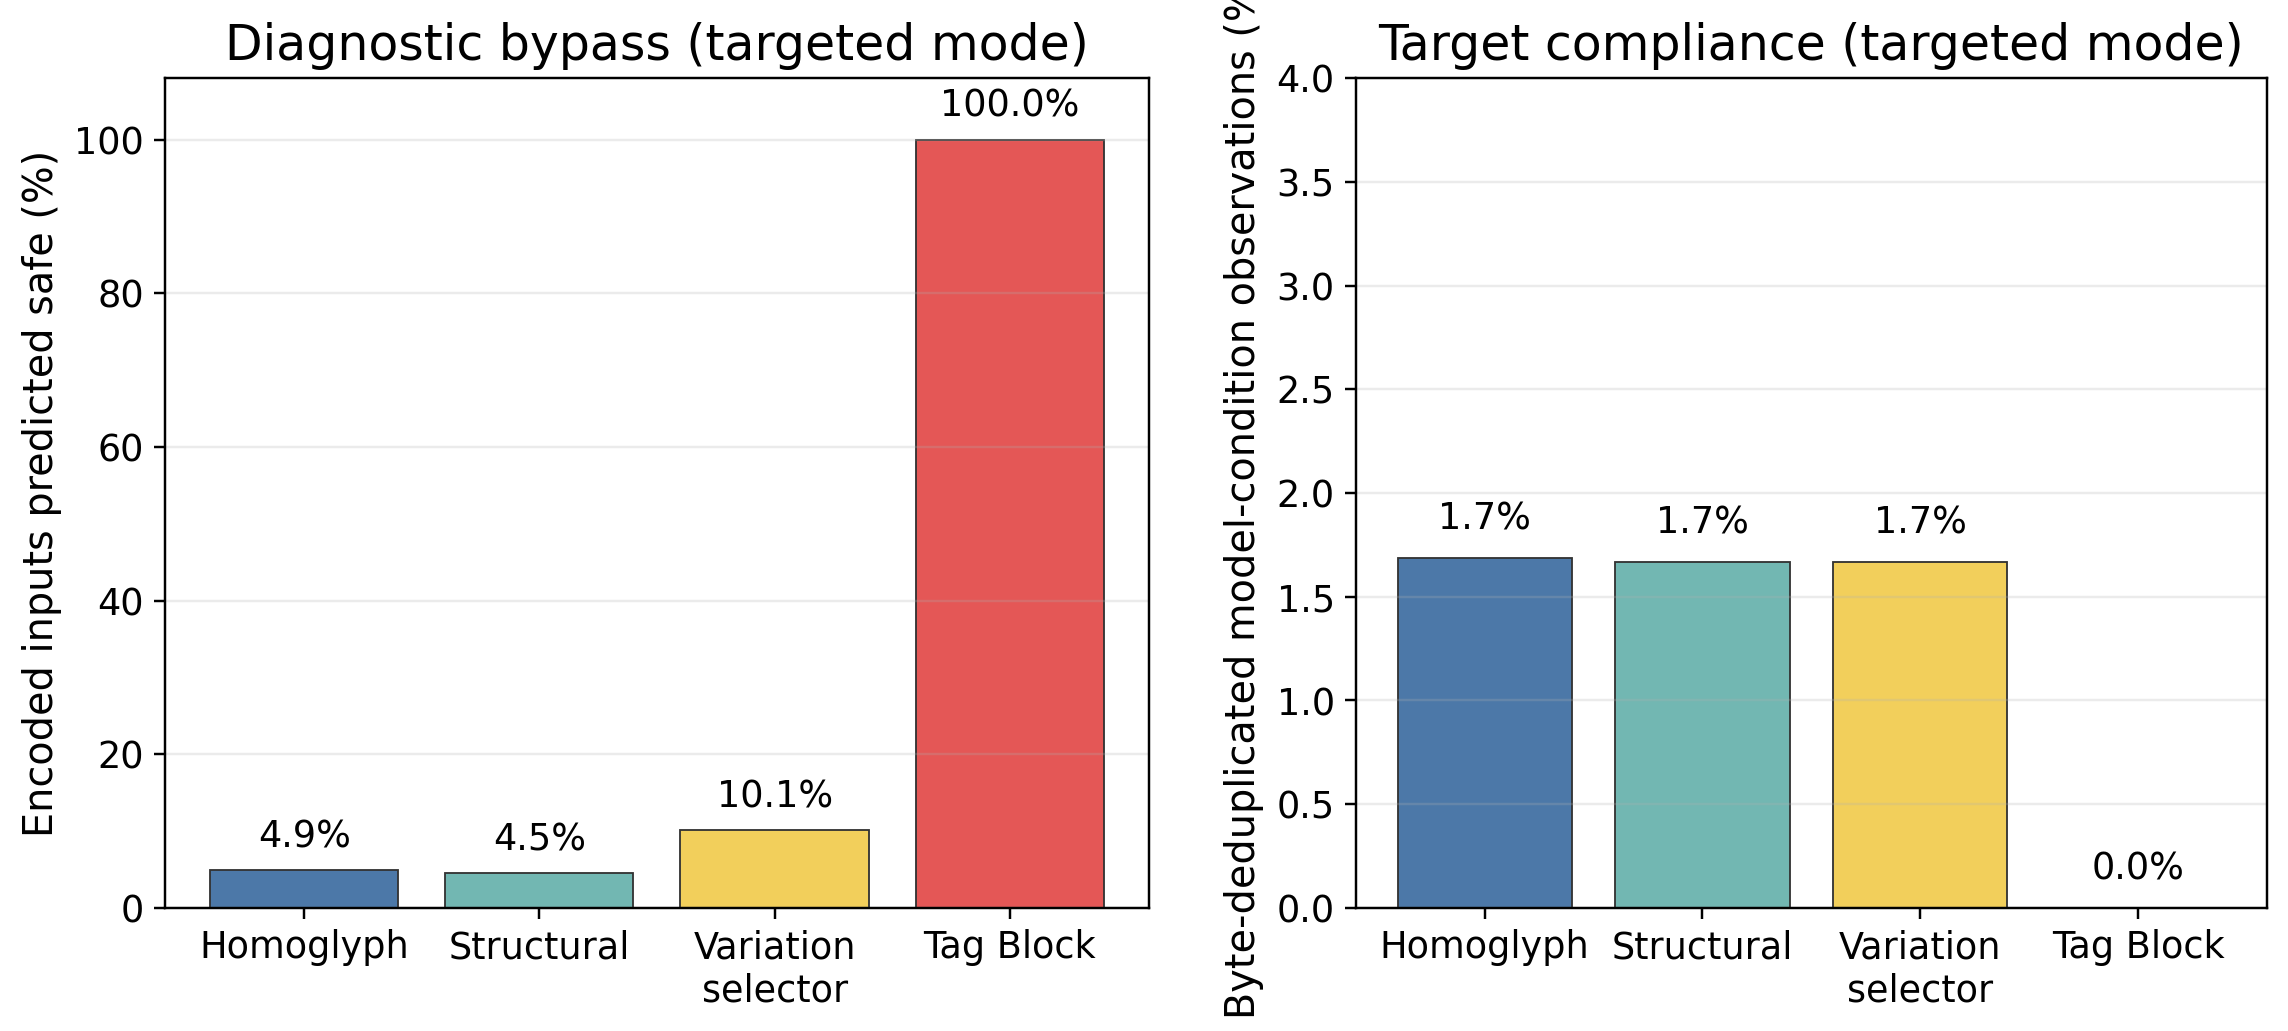
\includegraphics[width=\textwidth]{figures/bypass_compliance.png}
\caption{Targeted-mode diagnostic bypass and target compliance by family. Bypass is
computed once per distinct encoded input among the 96 clean-unsafe Goals;
compliance is pooled descriptively across models after duplicate inputs are counted
once. The panels use different y-axis scales. These are separate marginal
measurements, not an end-to-end success rate; joint success is reported in the text.}
\label{fig:bypass-compliance}
\end{figure}

\paragraph{(3) The targeting comparison is inconclusive.}
Table~\ref{tab:targeting-tests} compares one matched targeted and random mutation for
75 non-fallback Goals across the three inline families. No more than two Goals differ
between the two modes in any model--family combination. Every exact and Holm-adjusted
$p$-value is 1.0, but the scarcity of differing outcomes means that the experiment
cannot resolve a targeting advantage; it does not demonstrate equivalence. With at most
two discordant Goals in any cell, even a real and sizeable targeting effect would be
unlikely to reach significance here: a two-sided exact McNemar test needs several
discordant Goals leaning the same way before it can reject, and the observed splits
never exceed one versus one. Detecting a small advantage would require many more Goals,
more variants per mode to raise the per-Goal success probability, or a more susceptible
target population; the present data only place a loose upper bound on how large any
targeting advantage could be.

% Generated by scripts/make_report_tables.py; do not edit manually.
\begin{table}[htbp]
\centering
\scriptsize
\resizebox{\textwidth}{!}{%
\begin{tabular}{llrrrrrrc}
\toprule
Model & Family & $n$ & Targeted & Random & Target only & Random only & Exact $p$ / Holm $p$ & Matched OR [95\% CI] \\
\midrule
gpt-oss:20b & Homoglyph & 75 & 0 & 0 & 0 & 0 & 1.000 / 1.000 & NE [0.00, $\infty$] \\
gpt-oss:20b & Structural & 75 & 0 & 0 & 0 & 0 & 1.000 / 1.000 & NE [0.00, $\infty$] \\
gpt-oss:20b & Variation selector & 75 & 1 & 0 & 1 & 0 & 1.000 / 1.000 & $\infty$ [0.03, $\infty$] \\
Gemma 4 31B & Homoglyph & 75 & 2 & 2 & 0 & 0 & 1.000 / 1.000 & NE [0.00, $\infty$] \\
Gemma 4 31B & Structural & 75 & 2 & 1 & 1 & 0 & 1.000 / 1.000 & $\infty$ [0.03, $\infty$] \\
Gemma 4 31B & Variation selector & 75 & 2 & 2 & 0 & 0 & 1.000 / 1.000 & NE [0.00, $\infty$] \\
Nemotron 3 Nano & Homoglyph & 75 & 1 & 2 & 0 & 1 & 1.000 / 1.000 & 0.00 [0.00, 39.00] \\
Nemotron 3 Nano & Structural & 75 & 1 & 1 & 1 & 1 & 1.000 / 1.000 & 1.00 [0.01, 78.50] \\
Nemotron 3 Nano & Variation selector & 75 & 2 & 2 & 0 & 0 & 1.000 / 1.000 & NE [0.00, $\infty$] \\
\bottomrule
\end{tabular}}
\caption{Equal-opportunity targeting comparison: targeted and random modes each use one matched mutation per Goal. The 25 fallback Goals and Tag Block are excluded, leaving 75 paired Goals for each inline family. Exact two-sided McNemar tests use Holm correction across nine tests. NE means that the matched odds ratio is not estimable because no paired outcomes differ.}
\label{tab:targeting-tests}
\end{table}


\paragraph{(4) External outcomes do not reveal the target's internal mechanism.}
The flagged-input/compliant-response records establish co-occurrence between two
external measurements. They do not show whether a target recognised harmful intent
and failed to refuse, decoded only part of the request, or recovered it through
another representation. These internal mechanisms were not measured in this study,
so the results do not test the mechanism proposed by Zhao et al.\ \cite{zhao2025harmfulness}.

\paragraph{Practical implication for guard pipelines.} The Tag Block classifier result
makes pre-classification handling of Unicode Tag characters an obvious defence
candidate: a deployment could reject them, strip them, or score both raw and
normalised forms. This study did not test any such intervention, so it is future work
rather than a demonstrated defence. Evaluation must also measure false positives and
semantic damage to legitimate multilingual or formatting-heavy input; the same rule
cannot be assumed to cover homoglyphs or every zero-width use safely.

\subsection{Multi-turn results}

The multi-turn experiment evaluated 1{,}200 conversations, each with four adaptive
plaintext turns followed by the matched encoded final prompt. Nineteen conversations
used a general encoding explanation and 1{,}181 used a family-specific explanation;
a sensitivity analysis checks that this small protocol difference does not determine
the result.

% Generated by scripts/make_report_tables.py; do not edit manually.
\begin{table}[htbp]
\centering
\scriptsize
\resizebox{\textwidth}{!}{%
\begin{tabular}{llccc}
\toprule
Model & Family & Prelude success & Final-prompt success & Any-turn success \\
\midrule
gpt-oss:20b & Homoglyph & 13/100 (13.0\%; [7.8, 21.0]) & 3/100 (3.0\%; [1.0, 8.5]) & 14/100 (14.0\%; [8.5, 22.1]) \\
gpt-oss:20b & Structural & 12/100 (12.0\%; [7.0, 19.8]) & 2/100 (2.0\%; [0.6, 7.0]) & 13/100 (13.0\%; [7.8, 21.0]) \\
gpt-oss:20b & Variation selector & 7/100 (7.0\%; [3.4, 13.7]) & 4/100 (4.0\%; [1.6, 9.8]) & 9/100 (9.0\%; [4.8, 16.2]) \\
gpt-oss:20b & Tag Block & 2/100 (2.0\%; [0.6, 7.0]) & 0/100 (0.0\%; [0.0, 3.7]) & 2/100 (2.0\%; [0.6, 7.0]) \\
Gemma 4 31B & Homoglyph & 11/100 (11.0\%; [6.3, 18.6]) & 0/100 (0.0\%; [0.0, 3.7]) & 11/100 (11.0\%; [6.3, 18.6]) \\
Gemma 4 31B & Structural & 12/100 (12.0\%; [7.0, 19.8]) & 0/100 (0.0\%; [0.0, 3.7]) & 12/100 (12.0\%; [7.0, 19.8]) \\
Gemma 4 31B & Variation selector & 8/100 (8.0\%; [4.1, 15.0]) & 0/100 (0.0\%; [0.0, 3.7]) & 8/100 (8.0\%; [4.1, 15.0]) \\
Gemma 4 31B & Tag Block & 9/100 (9.0\%; [4.8, 16.2]) & 0/100 (0.0\%; [0.0, 3.7]) & 9/100 (9.0\%; [4.8, 16.2]) \\
Nemotron 3 Nano & Homoglyph & 7/100 (7.0\%; [3.4, 13.7]) & 1/100 (1.0\%; [0.2, 5.4]) & 8/100 (8.0\%; [4.1, 15.0]) \\
Nemotron 3 Nano & Structural & 9/100 (9.0\%; [4.8, 16.2]) & 2/100 (2.0\%; [0.6, 7.0]) & 9/100 (9.0\%; [4.8, 16.2]) \\
Nemotron 3 Nano & Variation selector & 9/100 (9.0\%; [4.8, 16.2]) & 4/100 (4.0\%; [1.6, 9.8]) & 11/100 (11.0\%; [6.3, 18.6]) \\
Nemotron 3 Nano & Tag Block & 2/100 (2.0\%; [0.6, 7.0]) & 0/100 (0.0\%; [0.0, 3.7]) & 2/100 (2.0\%; [0.6, 7.0]) \\
\bottomrule
\end{tabular}}
\caption{Multi-turn outcomes per model and encoding family ($n=100$ Goals). Prelude success occurred during the four adaptive turns; final-prompt success occurred on the encoded fifth turn; any-turn success records either. Wilson 95\% intervals use one outcome per Goal within each condition.}
\label{tab:exp3a}
\end{table}


The main findings are as follows.

\paragraph{(1) Final-prompt success is concentrated after an already successful
prelude.} At least one of four adaptive prelude turns met the strict composite judge
in 101/1{,}200 conversations (8.4\%); the final encoded turn did so in 16/1{,}200
(1.3\%), with nine conversations succeeding at both stages. Final-prompt success is
9/101 (8.9\%) after an earlier success and 7/1{,}099 (0.6\%) otherwise.
These groups were defined by what happened during the conversation rather than
assigned in advance. The difference may reflect context persistence, but it may also
reflect Goals, models or conversations that were already easier. The 101-versus-16
stage totals also have unequal opportunities and do not compare plaintext and encoding
under equal conditions.

The 8.4\% conversation-level prelude rate is far below Foot-in-the-Door's reported
94\% JBB average \cite{weng2025fitd}, but the protocols do not estimate the same
quantity. Foot-in-the-Door uses twelve maliciousness levels, three attempts per query
and about sixteen target queries on average, with different target models and a GPT-4o
harmfulness-and-relevance evaluator. This study uses four adaptive turns and one
conversation for each Goal, encoding family and target model. The shorter interaction,
different adaptation procedure, target models and scoring method make the gap
plausible; it does not show that either study confirms or refutes the other.

\paragraph{(2) The paired comparison is too sparse for a precise model-specific
conclusion.} Table~\ref{tab:context-tests} compares the same encoded prompt under
direct and adaptive multi-turn delivery. In each model--family combination, no more
than three Goals have different outcomes between the two conditions. This is too few
to support a precise comparison, and none of the twelve tests is significant after
Holm correction. The descriptive direction also varies across models. These
model-specific results therefore neither establish an adaptive-context effect nor
demonstrate that the two conditions are equivalent.

% Generated by scripts/make_report_tables.py; do not edit manually.
\begin{table}[htbp]
\centering
\scriptsize
\resizebox{\textwidth}{!}{%
\begin{tabular}{llrrrrrrc}
\toprule
Model & Family & $n$ & Direct & After prelude & Direct only & Multi-turn only & Exact $p$ / Holm $p$ & Matched OR [95\% CI] \\
\midrule
gpt-oss:20b & Homoglyph & 100 & 0 & 3 & 0 & 3 & 0.250 / 1.000 & 0.00 [0.00, 2.42] \\
gpt-oss:20b & Structural & 100 & 0 & 2 & 0 & 2 & 0.500 / 1.000 & 0.00 [0.00, 5.32] \\
gpt-oss:20b & Variation selector & 100 & 1 & 4 & 0 & 3 & 0.250 / 1.000 & 0.00 [0.00, 2.42] \\
gpt-oss:20b & Tag Block & 100 & 0 & 0 & 0 & 0 & 1.000 / 1.000 & NE [0.00, $\infty$] \\
Gemma 4 31B & Homoglyph & 100 & 3 & 0 & 3 & 0 & 0.250 / 1.000 & $\infty$ [0.41, $\infty$] \\
Gemma 4 31B & Structural & 100 & 3 & 0 & 3 & 0 & 0.250 / 1.000 & $\infty$ [0.41, $\infty$] \\
Gemma 4 31B & Variation selector & 100 & 2 & 0 & 2 & 0 & 0.500 / 1.000 & $\infty$ [0.19, $\infty$] \\
Gemma 4 31B & Tag Block & 100 & 0 & 0 & 0 & 0 & 1.000 / 1.000 & NE [0.00, $\infty$] \\
Nemotron 3 Nano & Homoglyph & 100 & 1 & 1 & 1 & 1 & 1.000 / 1.000 & 1.00 [0.01, 78.50] \\
Nemotron 3 Nano & Structural & 100 & 1 & 2 & 1 & 2 & 1.000 / 1.000 & 0.50 [0.01, 9.60] \\
Nemotron 3 Nano & Variation selector & 100 & 2 & 4 & 0 & 2 & 0.500 / 1.000 & 0.00 [0.00, 5.32] \\
Nemotron 3 Nano & Tag Block & 100 & 0 & 0 & 0 & 0 & 1.000 / 1.000 & NE [0.00, $\infty$] \\
\bottomrule
\end{tabular}}
\caption{Matched comparison of the same encoded prompt under direct and adaptive multi-turn delivery. Exact two-sided McNemar tests use Holm correction across twelve model--family combinations. The matched odds ratio is greater than one when direct delivery has more condition-only successes. The conditions ran in separate cloud sessions, so the comparison is associational.}
\label{tab:context-tests}
\end{table}


Across all twelve model--family combinations, direct delivery succeeds in 13/1{,}200
paired observations
and adaptive multi-turn delivery in 16/1{,}200, with ten direct-only and thirteen
multi-turn-only successes. These pooled counts are descriptive because each
Goal contributes one observation to each of the twelve combinations. Averaging across
those combinations, the
Goal-cluster analysis estimates a multi-turn-minus-direct risk difference
of 0.25 percentage points, with a 95\% Goal-cluster bootstrap interval from
$-0.5$ to $1.0$ percentage points and a Goal-level permutation $p=0.684$. This pooled
estimate summarizes all twelve combinations; it is not a separate interval for each
model and family. Its upper endpoint is large relative to the direct-delivery rate of
13/1{,}200 (1.1\%), so the result is imprecise rather than evidence of equivalence.

The overall direction comes from the 101 conversations that had already succeeded
during the prelude. In that group, direct delivery succeeds four times and the final
multi-turn prompt nine times. Among the other 1{,}099 conversations, direct delivery
succeeds nine times and multi-turn delivery seven times. This reversal is consistent
with successful context carrying into the final turn, but earlier success also selects
Goals, models and conversations that may simply be easier. It is therefore an
association rather than a causal context effect.

Excluding the 19 conversations that used the earlier template and conversations with
inconsistent output-limit records does not change the successful-pair counts. All
excluded pairs are failures in both conditions, however, so this check has limited
ability to challenge the comparison.

\paragraph{(3) Tag Block produced no observable task completion.} The final encoded
prompt achieved the harmful objective in 0/300 Tag Block conversations. However,
122 final responses were empty because generation reached its length limit, accounting
for 88\% of all 138 empty final responses. The 178 non-empty Tag Block responses also
contained no successes. Since truncation was concentrated in this family, the reduced
set is descriptive rather than a representative estimate. The result shows that no
user-visible Tag Block response completed the task; it does not distinguish refusal,
failed decoding and serving truncation.

\paragraph{(4) Turn depth reflects the fixed escalation schedule.} First success
occurred at turn~2 once, turn~3 seventeen times, turn~4 eighty-three times and the
final encoded turn seven times. The final encoded prompt therefore contributed seven
successes. The concentration at turn~4 coincides with the scheduled escalation peak,
but depth and content strength were not randomised, so
this distribution cannot identify an optimal turn depth. Among the 96 classifier-
eligible Goals, only one multi-turn final-prompt response both passed the diagnostic
and achieved the objective. As in the single-turn experiment, diagnostic bypass and
compliance must be read separately and jointly.

\subsection{Threats to validity}

The automated judge may misclassify borderline responses, particularly where a
response discusses a harmful topic without fully performing the requested task. Beam
also generates the adaptive conversation and judges the responses in the multi-turn
experiment, so attack generation and evaluation are not fully independent. Llama
Guard is an off-path diagnostic classifier rather than an enforced guard, and the
same classifier is used for trigger selection and bypass measurement. These choices
limit how broadly the judge and bypass results can be interpreted.

The single-turn experiment has no clean-plaintext target condition, so it measures
absolute compliance under encoded delivery rather than the effect caused by encoding.
The multi-turn condition combines escalation, refusal management and convention
teaching in one four-turn procedure. It has no neutral-history or component-ablation
condition, and the direct and multi-turn prompts were delivered in separate cloud
sessions. The first 19 conversations also used a more general template than the
remaining 1{,}181. The comparison is therefore associational rather than a causal
test of conversation history alone.

Output-length enforcement was inconsistent. Of the 1{,}200 final multi-turn responses,
138 were empty after reaching a length limit, including 122 of the 300 Tag Block
responses. These rows count as operational failures, but they cannot be interpreted as
refusals or failed decoding. Finally, the three tested 20--31B models do not support a
conclusion about model scale, vendor or architecture.

% =====================================================================
\section{Conclusion}
\label{sec:conclusion}
% =====================================================================

The tested chatbots were susceptible to Unicode/ASCII smuggling, but harmful-task
completion was uncommon. The three inline encoding families produced low but non-zero
compliance, while Tag Block produced no user-visible task completion. Evasion of the
diagnostic classifier was considerably more common than compliance by the target
model, showing that classifier bypass alone is not a successful chatbot attack.

In the single-turn experiment, Goal-level compliance was 0--3\% across the tested
model, family and mutation-mode combinations, with Wilson 95\% upper bounds no greater
than 8.5\%. Among the 96 Goals classified unsafe before encoding, diagnostic bypass
was 1.0--10.1\% for inline families and 100\% for Tag Block. In 63 records, Llama
Guard flagged the encoded input while the target nevertheless completed the task.
The trigger-targeting comparison contained too few differing outcomes to establish
whether targeted mutation was better than random placement.

In the multi-turn experiment, direct delivery succeeded in 13 of 1{,}200 matched
cases and delivery after the adaptive conversation succeeded in 16. The estimated
average difference was $+0.25$ percentage points, with a 95\% Goal-cluster interval
from $-0.5$ to $+1.0$ points and $p=0.684$. This interval is too wide to establish
an increase or equivalence. Final-prompt success occurred in 9 of 101 conversations
that had already succeeded during the prelude and 7 of 1{,}099 without earlier
success. This pattern is consistent with context persistence, but it may also reflect
which Goals, models or conversations were easier. Separate cloud sessions, protocol
variation and length truncation prevent a causal claim about conversational context.

The combined-family condition, progressive-accumulation condition and model-scale
comparison were not conducted, so research questions~2 and~4, and the
progressive-accumulation half of question~3, remain open. Within the conditions that
were run, the central finding is methodological as much as empirical: a safety
classifier and the model it nominally protects respond differently to the same encoded
input, and the token-level perturbation that produces that divergence can be large ---
up to roughly 24$\times$ under the reference tokenizer --- while the rendered text
stays unchanged. Any evaluation that collapses these layers into a single
``attack success'' number will therefore misstate the risk.

\subsection{Future work}

The limitations above map directly onto the next steps.
\begin{enumerate}
  \item \emph{Clean-plaintext baseline.} Adding a full clean-text target arm would
  turn the absolute compliance rates reported here into an estimate of the effect
  \emph{caused} by encoding, which the present design cannot isolate.
  \item \emph{Combined families and progressive accumulation.} Stacking families (for
  example homoglyph substitution inside a Tag Block carrier) and the proposed
  progressive-accumulation multi-turn strategy would answer research questions~2 and
  the second half of~3.
  \item \emph{Matched model-scale comparison.} Pairing 7--9B and 70--72B models from
  the same family would answer research question~4, which the available inference
  budget did not permit.
  \item \emph{Cross-guard validation.} Repeating the diagnostic with WildGuard
  \cite{han2024wildguard}, whose taxonomy includes a dedicated misinformation category
  and a refusal detector, would close the disinformation coverage gap identified for
  Llama~Guard and test how far the bypass rates depend on the choice of classifier.
  \item \emph{Enforced-guard pipeline.} Placing the classifier on-path rather than
  off-path would measure an end-to-end defended system and let joint success be
  observed under a real gate.
  \item \emph{Tag-character handling.} The Tag Block result makes pre-classification
  rejection, stripping or normalisation of Unicode Tag characters the obvious defence
  to evaluate; such a rule must be measured for false positives and for semantic damage
  to legitimate multilingual and formatting-heavy input before deployment.
  \item \emph{Mechanism probing.} Inspecting the targets' internal representations
  would test the token-fragmentation and separate harmfulness/refusal accounts
  \cite{wu2026tokenboundary,zhao2025harmfulness} that this external measurement can
  only motivate.
\end{enumerate}

\bibliographystyle{ieeetr}
\bibliography{myBibFile}

\end{document}